% === T08 - Lenguaje Ensamblador ===
% David Alejandro Gonzalez Marquez
% fokerman@gmail.com
% https://github.com/fokerman/computingSystemsCourse

\documentclass[aspectratio=169]{beamer}
\usepackage{../packages}

\title{\Huge Lenguaje Ensamblador}
\author{David Alejandro González Márquez}
\institute{}

\date{}

\begin{document}

\begin{frame}[plain]
    \titlepage
    \begin{textblock}{100}(30,80)
    \begin{tcolorbox}[size=small,width=\textwidth,colback={gray!30},title={}]
    \begin{center}
     \scriptsize Clase disponible en: \url{https://github.com/fokerman/computingSystemsCourse}
    \end{center}
    \end{tcolorbox}
    \end{textblock}
%     \begin{textblock}{140}(10,70)
%     \textcolor{rojo}{
%     \textbf{Atención}: La clase será grabada por el anfitrión para su posterior y eventual uso académico dentro de nuestra institución. Su participación en la clase implica brindar su consentimiento para participar en la grabación, aunque pueden mantener su video apagado.}
%     \end{textblock}
\end{frame}

\begin{frame}[fragile]{Lenguaje Ensamblador}
    \begin{textblock}{80}(10,15)
    El lenguaje ensamblador consiste en escribir las instrucciones del procesador como \textbf{texto} (mnemónicos).\\
    \bigskip
    Estas instrucciones son convertidas a su codificación binaria por medio del \textbf{ensamblador}.\\
    \bigskip
    Los lenguajes de tipo ensamblador, son \textbf{específicos} para cada arquitectura.\\
    \bigskip
    Los mnemónicos que pueden ser escritos dependen de las instrucciones que soporte el procesador.
    \end{textblock}
    \begin{textblock}{140}(10,75)
    \textcolor{verdeuca}{En lo que sigue, vamos a estudiar el lenguaje ensamblador de la arquitectura \texttt{x86-64} o \texttt{AMD64}.}
    \end{textblock}
    \begin{textblock}{70}(95,15) \only<1->{
\includegraphics[scale=1.7]{img/ensambladores.pdf}} \end{textblock}
\end{frame}

\begin{frame}[fragile]{Arquitectura \texttt{x86-64} o \texttt{AMD64}}
    \begin{itemize}
    \setlength\itemsep{0.5cm}
    \item[-] Es una \textbf{extensión} de la arquitectura \texttt{x86} de Intel.
    \item[-] Binario \textbf{compatible} con toda la línea de procesadores.
    \item[-] Desarrollado por AMD bajo el nombre \textbf{AMD64}.
    \item[-] Vio la luz en el 2003 bajo la línea de procesadores \texttt{Opteron}.
    \item[-] Actualmente es el estándar en notebooks, computadoras de escritorio y servidores.
    \item[-] Compite con arquitecturas como ARM y sus extensiones, enfocadas principalmente a dispositivos embebidos*.
    \end{itemize}
\end{frame}

\begin{frame}[fragile]{Arquitectura \texttt{x86-64} o \texttt{AMD64}}
    \textit{Características:}\\
    \begin{itemize}
    \item[-] Arquitectura de 64 bits.
    \item[-] Direcciones de memoria de 64 bits (8 bytes), direccionable a byte.
    \item[-] Registros de 64 bits (pueden operar también en 32, 16 u 8 bits).
    \item[-] Opera con datos en \textit{little endian}.
    \item[-] Múltiples modos de direccionamiento.
    \end{itemize}
    \pause
    \textit{Manuales:}\\
    \begin{itemize}
    \item[-] Intel $^{\circledR}$ 64 and IA-32 Architectures - Software Developer’s Manual\\
    \begin{itemize}
    \item[-] Volume 1: Basic Architecture.
    \item[-] Volume 2: Instruction Set Reference A-Z.
    \item[-] Volume 3: System Programming.
    \item[-] Volume 4: Model-Specific Registers.
    \end{itemize}
    Total 4778 páginas.\\
    { \scriptsize \url{https://software.intel.com/content/www/us/en/develop/articles/intel-sdm.html} }\\
    \end{itemize}
\end{frame}

\begin{frame}[fragile,t]{Arquitectura \texttt{x86-64} o \texttt{AMD64}}{Registros}
    \begin{textblock}{70}(8,15)
    \small Conjuntos de Registros:
    \begin{enumerate}
    \item \only<1|handout:0>{Registros de propósito general}\only<2->{\textbf{Registros de propósito general}}
    \item \only<1|handout:0>{Registros de la unidad de Punto Flotante}\only<2->{\sout{Registros de la unidad de Punto Flotante}}
    \item \only<1|handout:0>{Registros de las extensiones MMX}\only<2->{\sout{Registros de las extensiones MMX}}
    \item \only<1|handout:0>{Registros de las extensiones SSE}\only<2->{\sout{Registros de las extensiones SSE}}
    \end{enumerate}
    \only<2->{\textcolor{verdeuca}{Vamos a hacer foco solo sobre los registros\\ de \textbf{propósito general}.}}
    \end{textblock}
    \begin{textblock}{70}(15,60) \only<2->{\includegraphics[scale=1.2]{img/regSize-layer1.pdf}} \end{textblock}
    \begin{textblock}{70}(15,60) \only<3->{\includegraphics[scale=1.2]{img/regSize-layer2.pdf}} \end{textblock}
    \begin{textblock}{70}(15,60) \only<4->{\includegraphics[scale=1.2]{img/regSize-layer3.pdf}} \end{textblock}
    \begin{textblock}{70}(15,60) \only<5->{\includegraphics[scale=1.2]{img/regSize-layer4.pdf}} \end{textblock}
    \begin{textblock}{70}(78,10) \only<2->{\includegraphics[scale=0.85]{img/regName-layer1.pdf}} \end{textblock}
    \begin{textblock}{70}(78,10) \only<3->{\includegraphics[scale=0.85]{img/regName-layer2.pdf}} \end{textblock}
    \begin{textblock}{70}(78,10) \only<4->{\includegraphics[scale=0.85]{img/regName-layer3.pdf}} \end{textblock}
    \begin{textblock}{70}(78,10) \only<5->{\includegraphics[scale=0.85]{img/regName-layer4.pdf}} \end{textblock}
\end{frame}

\begin{frame}[fragile,t]{Arquitectura \texttt{x86-64} o \texttt{AMD64}}{Parámetros}
    \small
    Las instrucciones en general pueden tomar entre tres y cero parámetros.\\
    Sus posibilidades son las siguientes:\\
    \begin{textblock}{65}(10,27)
    \only<2->{
    \textbf{Implícito}\\
    \footnotesize El operando es parte de la instrucción.\\
    \hspace{0.5cm} \textcolor{gray}{Ej.} \hspace{0.3cm} \textcolor{verdeuca}{\texttt{CLC}, clear carry flag.}
    }
    \end{textblock}
    \begin{textblock}{70}(10,45)
    \only<3->{
    \textbf{Inmediato}\\
    \footnotesize Un valor constante inmediato como parte de la codificación de la instrucción.\\
    \hspace{0.5cm} \textcolor{gray}{Ej.} \hspace{0.3cm} \textcolor{verdeuca}{\texttt{MOV RAX, 150}}
    }
    \end{textblock}
    \begin{textblock}{65}(10,67)
    \only<4->{
    \textbf{Registro}\\
    \footnotesize Un registro de propósito general u otros registros según la instrucción.\\
    \hspace{0.5cm} \textcolor{gray}{Ej.} \hspace{0.3cm} \textcolor{verdeuca}{\texttt{ADD AX, BX}}
    }
    \end{textblock}
    \begin{textblock}{70}(80,27)
    \only<5->{
    \textbf{Memoria}\\
    \footnotesize Una dirección de memoria respetando el formato:\\
    \vspace{-0.2cm}
    \begin{center}
    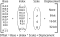
\includegraphics[scale=0.8]{img/addressMode64.pdf}
    \end{center}
    \vspace{-0.2cm}
    \hspace{0.5cm} \textcolor{gray}{Ej.} \hspace{0.3cm} \textcolor{verdeuca}{\texttt{ADD AL, [0x123123]}}\\
    \hspace{0.5cm} \textcolor{gray}{Ej.} \hspace{0.3cm} \textcolor{verdeuca}{\texttt{ADD AX, [RDX]}}\\
    \hspace{0.5cm} \textcolor{gray}{Ej.} \hspace{0.3cm} \textcolor{verdeuca}{\texttt{ADD EAX, [RBX+RCX]}}\\
    \hspace{0.5cm} \textcolor{gray}{Ej.} \hspace{0.3cm} \textcolor{verdeuca}{\texttt{ADD RAX, [RBX+RCX*2+5]}}\\
    }
    \end{textblock}
\end{frame}

\begin{frame}[fragile]{Arquitectura \texttt{x86-64} o \texttt{AMD64}}{Conjunto de Instrucciones (algunas)}
    \begin{tabular}{p{2.7cm}|p{10cm}}
    Instrucción & Descripción \\ \hline
    \texttt{ADD DST, SRC} & \textcolor{verdeuca}{\texttt{DST = DST + SRC}                       }\\
    \texttt{ADC DST, SRC} & \textcolor{verdeuca}{\texttt{DST = DST + SRC + carry}               }\\
    \texttt{SUB DST, SRC} & \textcolor{verdeuca}{\texttt{DST = DST - SRC}                       }\\
    \texttt{SBB DST, SRC} & \textcolor{verdeuca}{\texttt{DST = DST - SRC - borrow}              }\\
    \texttt{INC DST}      & \textcolor{verdeuca}{\texttt{DST = DST + 1}                         }\\
    \texttt{DEC DST}      & \textcolor{verdeuca}{\texttt{DST = DST - 1}                         }\\
    \texttt{NEG DST}      & \textcolor{verdeuca}{\texttt{DST = -DST}                            }\\
    \texttt{CMP DST, SRC} & \textcolor{verdeuca}{Altera los flags resultado de \texttt{DST-SRC} }\\ \hline                  
    \texttt{AND DST, SRC} & \textcolor{verdeuca}{\texttt{DST = bitwiseAnd(DST, SRC)}            }\\
    \texttt{OR  DST, SRC} & \textcolor{verdeuca}{\texttt{DST = bitwiseOr(DST, SRC)}             }\\
    \texttt{XOR DST, SRC} & \textcolor{verdeuca}{\texttt{DST = bitwiseXor(DST, SRC)}            }\\
    \texttt{NOT DST}      & \textcolor{verdeuca}{\texttt{DST = bitwiseNot(DST)}                 }\\
    \hline
    \end{tabular}
\end{frame}

% \begin{frame}[fragile]{Arquitectura \texttt{x86-64} o \texttt{AMD64}}{Conjunto de Instrucciones (algunas)}
% \begin{tabular}{p{2.7cm}|p{10cm}}
% Instrucción & Descripción \\ \hline
% \texttt{IMUL} Signed multiply.
% \texttt{MUL} Unsigned multiply.
% \texttt{IDIV} Signed divide.
% \texttt{DIV REG}      & División sin signo de RDX:RAX por REG. RAX=Resultado, RDX=Resto.
% \end{tabular}
% \end{frame}

\begin{frame}[fragile]{Arquitectura \texttt{x86-64} o \texttt{AMD64}}{Conjunto de Instrucciones (algunas)}
    \begin{tabular}{p{2.7cm}|p{10cm}}
    Instrucción & Descripción \\ \hline
    \texttt{SAR DST, imm} & \textcolor{verdeuca}{Shift aritmético a derecha     }\\
    \texttt{SHR DST, imm} & \textcolor{verdeuca}{Shift lógico a derecha         }\\
    \texttt{SAL DST, imm} & \textcolor{verdeuca}{Shift aritmético a izquierda   }\\
    \texttt{SHL DST, imm} & \textcolor{verdeuca}{Shift lógico a izquierda       }\\
    \texttt{ROR DST, imm} & \textcolor{verdeuca}{Rotación a derecha             }\\
    \texttt{ROL DST, imm} & \textcolor{verdeuca}{Rotación a izquierda           }\\
    \texttt{RCR DST, imm} & \textcolor{verdeuca}{Rotación con carry a derecha   }\\
    \texttt{RCL DST, imm} & \textcolor{verdeuca}{Rotación con carry a izquierda }\\
    \end{tabular}\\
    \bigskip
    \begin{tabular}{p{2.7cm}|p{10cm}}
    Instrucción & Descripción \\ \hline
    \texttt{XCHG DST, SRC} & \textcolor{verdeuca}{Intercambia dos datos, ya sea memoria o registros}\\
    \texttt{MOV DST, SRC}  & \textcolor{verdeuca}{Copia datos entre registros, memoria o setea valores inmediatos}\\
    \end{tabular}
\end{frame}

\begin{frame}[fragile]{Arquitectura \texttt{x86-64} o \texttt{AMD64}}{Conjunto de Instrucciones (algunas)}
    \begin{tabular}{p{2.7cm}|p{10cm}}
    Instrucción & Descripción \\ \hline
    \texttt{JMP DST}  & \textcolor{verdeuca}{Salto incondicional          }\\
    \texttt{JE DST}   & \textcolor{verdeuca}{Salto si es igual            }\\ %JNE
    \hline
    \texttt{JA  DST} & \textcolor{verdeuca}{Salto si es $>$ (sin signo)   }\\ %JNBE
    \texttt{JAE DST} & \textcolor{verdeuca}{Salto si es $\ge$ (sin signo) }\\ %JNB
    \texttt{JB  DST} & \textcolor{verdeuca}{Salto si es $<$ (sin signo)   }\\ %JNAE
    \texttt{JBE DST} & \textcolor{verdeuca}{Salto si es $\le$ (sin signo) }\\ %JNA
    \hline
    \texttt{JG  DST} & \textcolor{verdeuca}{Salto si es $>$ (con signo)   }\\ %JNLE
    \texttt{JGE DST} & \textcolor{verdeuca}{Salto si es $\ge$ (con signo) }\\ %JNL 
    \texttt{JL  DST} & \textcolor{verdeuca}{Salto si es $<$ (con signo)   }\\ %JNGE
    \texttt{JLE DST} & \textcolor{verdeuca}{Salto si es $\le$ (con signo) }\\ %JNG
    \hline
    \texttt{JC  DST} & \textcolor{verdeuca}{Salto si hay carry            }\\ %JNC
    \texttt{JO  DST} & \textcolor{verdeuca}{Salto si hay overflow         }\\ %JNO
    \texttt{JS  DST} & \textcolor{verdeuca}{Salto si es negativo          }\\ %JNS
    \texttt{JZ  DST} & \textcolor{verdeuca}{Salto si es cero              }\\ %JNZ
    \end{tabular}
\end{frame}

\begin{frame}[t]{Hola Mundo ...}
    \begin{block}{Ejemplo}
    Escribir un programa en lenguaje ensamblador que imprima por pantalla:\\
    \begin{center}
    \Large
    \texttt{Hola Mundo}
    \end{center}
    \vspace{.2cm}
    \end{block}
    \vspace{0.7cm}
    \pause
    \begin{center}
    \Huge ¿Cómo?
    \end{center}
\end{frame}

\begin{frame}[fragile]{Secciones, etiquetas y símbolos}
    Un programa se separa en secciones:\\
    \begin{itemize}
    \item \normalsize \textbf{section .data}: donde se declaran las variables globales inicializadas. \small (\texttt{DB}, \texttt{DW}, \texttt{DD} y \texttt{DQ}).
    \item \normalsize \textbf{section .text}: donde se escribe el código.
%     \item[-] \normalsize \texttt{.rodata}: Donde declarar constantes globales inicializadas. \small (\texttt{DB}, \texttt{DW}, \texttt{DD} y \texttt{DQ}).
%     \item[-] \normalsize \texttt{.bss}: Donde declarar variables globales no inicializadas. \small (\texttt{RESB}, \texttt{RESW}, \texttt{RESD} y \texttt{RESQ}).
    \end{itemize}
    \pause
    Etiquetas y símbolos:\\
    \begin{itemize}
        \item \textbf{\_start}: Símbolo utilizando como punto de entrada de un programa.
        \item \textbf{global}: Modificador que define un símbolo que va a ser visto externamente.
    \end{itemize}
    \pause
    Comandos e instrucciones para el ensamblador:\\
    \begin{itemize}
    \item \textbf{DB} define un byte, \textbf{DW} define una word (2 bytes), \textbf{DD} define una doble word (4 bytes),\\ \textbf{DQ} define una quad word (8 bytes). % \texttt{RESB}, \texttt{RESW}, \texttt{RESD} y \texttt{RESQ}.
    \item Expresión \textbf{\texttt{\$}}: toma el valor de la posición en memoria de la línea que contiene la expresión.
    \item Comando \textbf{EQU}: para definir constantes como ecuaciones que evalúa el ensamblador.
%     \item[-] comando \verb|INCBIN|, incluye un binario en un archivo assembler.
%     \item[-] prefijo \verb|TIMES|, repite una cantidad de veces la instrucción que le sigue.
    \end{itemize}
\end{frame}

\begin{frame}[fragile]{Llamadas al sistema operativo (syscalls)}
    Si vamos a querer imprimir en pantalla dentro de un sistema,\\
    tenemos que \textbf{solicitar permiso} al sistema operativo para hacerlo.\\
    \bigskip
    \pause
    En sistemas POSIX, como Linux, su interfaz es:
    \small
    \begin{enumerate}
    \item[1-] El número de función que queremos en RAX.
    \item[2-] Los parámetros en RBX, RCX, RDX, RSI, RDI y RBP; en ese orden.
    \item[3-] Llamamos a la interrupción del sistema operativo (int 0x80).
    \item[4-] En general, la respuesta está en RAX.
    \end{enumerate}
    \pause
    \begin{itemize}
    \item[-] \textcolor{verdeuca}{Mostrar por pantalla} (\textbf{sys\_write}):\\
    \begin{tabular}{l}
    Función \textbf{4}\\
    Parámetro 1: \textbf{¿donde?} (1 = stdout)\\
    Parámetro 2: \textbf{Dirección de memoria del mensaje}\\
    Parámetro 3: \textbf{Longitud del mensaje} (en bytes)\\
    \end{tabular}
    \pause
    \item[-] \textcolor{verdeuca}{Terminar programa} (\textbf{exit}):\\
    \begin{tabular}{l}
    Función \textbf{1}\\
    Parámetro 1: \textbf{código de retorno} (0 = sin error)\\
    \end{tabular}
    \end{itemize}
\end{frame}

\newcommand{\A}[0]{\begin{tikzpicture} \draw[white] (0,0) rectangle (.4,.4); \draw[white] (0,0) rectangle (.3,.3);\end{tikzpicture}}
\newcommand{\T}[0]{
\begin{tikzpicture} \draw[white] (0,0) rectangle (.4,.4); \draw[red,fill=red] (0,0) rectangle (.3,.3);\end{tikzpicture}}
\newcommand{\R}[0]{\begin{tikzpicture} \draw[white] (0,0) rectangle (.4,.4); \draw[verdeuca,fill=verdeuca] (0,0) rectangle (.3,.3);\end{tikzpicture}}
\newcommand{\B}[0]{\begin{tikzpicture} \draw[white] (0,0) rectangle (.4,.4); \draw[naranjauca,fill=naranjauca] (0,0) rectangle (.3,.3);\end{tikzpicture}}

\begin{frame}[fragile]{Hola Mundo...}
    \verb|     section .data                  |\\ 
    \verb|       msg: DB 'Hola Mundo', 10     | \A \\
    \verb|       largo EQU $ - msg            |\\
    \verb|                                    |\\
    \verb|       global _start                |\\
    \verb|     section .text                  |\\
    \verb|       _start:                      |\\
    \verb|         mov rax, 4     ; funcion 4 | \A \\
    \verb|         mov rbx, 1     ; stdout    | \A \\
    \verb|         mov rcx, msg   ; mensaje   | \A \\
    \verb|         mov rdx, largo ; longitud  | \A \\
    \verb|         int 0x80                   | \A \\
    \verb|         mov rax, 1     ; funcion 1 | \A \\
    \verb|         mov rbx, 0     ; codigo    | \A \\
    \verb|         int 0x80                   | \A \\
\end{frame}                          

\begin{frame}[fragile]{Hola Mundo...}
    \verb|     section .data                  |\\ 
    \verb|       msg: DB 'Hola Mundo', 10     | \A \A \B \B \B \B \B \B \B \B \B \B \T \\
    \verb|       largo EQU $ - msg            |\\
    \verb|                                    |\\
    \verb|       global _start                |\\
    \verb|     section .text                  |\\
    \verb|       _start:                      |\\
    \verb|         mov rax, 4     ; funcion 4 | \A \A  \R \R \B \B \B \B \B \B \B \B \\
    \verb|         mov rbx, 1     ; stdout    | \A \A  \R \R \B \B \B \B \B \B \B \B \\
    \verb|         mov rcx, msg   ; mensaje   | \A \A  \R \R \B \B \B \B \B \B \B \B \\
    \verb|         mov rdx, largo ; longitud  | \A \A  \R \R \B \B \B \B \B \B \B \B \\
    \verb|         int 0x80                   | \A \A  \R \B \\
    \verb|         mov rax, 1     ; funcion 1 | \A \A  \R \R \B \B \B \B \B \B \B \B \\
    \verb|         mov rbx, 0     ; codigo    | \A \A  \R \R \B \B \B \B \B \B \B \B \\
    \verb|         int 0x80                   | \A \A  \R \B \\
    \begin{textblock}{70}(90,22) \only<2->{ \small
    \textcolor{verdeuca}{¿Cómo funciona \textbf{EQU}?}\\
    \texttt{largo = 11 - 0}\\
    \texttt{largo = 11}\\
    } \end{textblock}
\end{frame}

\begin{frame}[fragile]{Hola Mundo...}
    \verb|     section .data                  |\\ 
    \verb|       msgPepe: DB 'Hola Pepe', 10  | \A \A \B \B \B \B \B \B \B \B \B \T \\
    \verb|       msg: DB 'Hola Mundo', 10     | \A \A \B \B \B \B \B \B \B \B \B \B \T \\
    \verb|       largo EQU $ - msg            |\\
    \verb|                                    |\\
    \verb|       global _start                |\\
    \verb|     section .text                  |\\
    \verb|       _start:                      |\\
    \verb|         mov rax, 4     ; funcion 4 | \A \A  \R \R \B \B \B \B \B \B \B \B \\
    \verb|         mov rbx, 1     ; stdout    | \A \A  \R \R \B \B \B \B \B \B \B \B \\
    \verb|         mov rcx, msg   ; mensaje   | \A \A  \R \R \B \B \B \B \B \B \B \B \\
    \verb|         mov rdx, largo ; longitud  | \A \A  \R \R \B \B \B \B \B \B \B \B \\
    \verb|         int 0x80                   | \A \A  \R \B \\
    \verb|         mov rax, 1     ; funcion 1 | \A \A  \R \R \B \B \B \B \B \B \B \B \\
    \verb|         mov rbx, 0     ; codigo    | \A \A  \R \R \B \B \B \B \B \B \B \B \\
    \verb|         int 0x80                   | \A \A  \R \B \\
    \begin{textblock}{70}(90,25) \only<2->{ \small
    \textcolor{verdeuca}{¿Cómo funciona \textbf{EQU}?}\\
    \texttt{largo = 21 - 10}\\
    \texttt{largo = 11}\\
    } \end{textblock}
\end{frame}  

\begin{frame}[fragile]{Ensamblando y linkeando}
    \textbf{Ensamblamos:}\\
    \vspace{0.2cm}
    \verb|      nasm -f elf64 -g -F DWARF holamundo.asm|\\
    \vspace{1cm}
    \textbf{Linkeamos:}\\
    \vspace{0.2cm}
    \verb|      ld -o holamundo holamundo.o|\\
    \vspace{1cm}
    \textbf{Ejecutamos:}\\
    \vspace{0.2cm}
    \verb|      ./holamundo|\\
\end{frame}

\begin{frame}[fragile]{Pila (Stack)}
    \begin{textblock}{65}(10,15)
    \uncover<1->{La Pila o Stack es una \textbf{estructura} en memoria administrada por el procesador.\\}
    \bigskip
    \uncover<1->{Se utiliza para guardar el \textbf{contexto de ejecución} de una función, variables locales y datos.\\}
    \bigskip
    \uncover<2->{En x86-64, se identifica por dos registros:\\}% \texttt{RBP} y \texttt{RSP}.\\
    \bigskip
    \begin{itemize}
    \item<2-> \texttt{RBP} - \textbf{Base Pointer}\\ Apunta a la base
    \item<2-> \texttt{RSP} - \textbf{Stack Pointer}\\ Al tope (último elemento válido)
    \end{itemize}
    \end{textblock}
    \begin{textblock}{70}(79,8) \only<2->{\includegraphics[scale=0.5]{img/pila-layer1.pdf}} \end{textblock} % pila 
    \begin{textblock}{70}(79,8) \only<3->{\includegraphics[scale=0.5]{img/pila-layer2.pdf}} \end{textblock} % flecha
    \begin{textblock}{70}(79,8) \only<2->{\includegraphics[scale=0.5]{img/pila-layer3.pdf}} \end{textblock} % rsp rbp
    \begin{textblock}{70}(79,8) \only<3->{\includegraphics[scale=0.5]{img/pila-layer4.pdf}} \end{textblock} % rangos
    \begin{textblock}{70}(79,8) \only<1->{\includegraphics[scale=0.5]{img/pila-layer5.pdf}} \end{textblock} % memoria
\end{frame}

\begin{frame}[fragile,t]{Pila (Stack)}
    \uncover<1->{Existen varias instrucciones que utilizan la pila, vamos a hacer foco en 4 de ellas.\\}
    \begin{textblock}{50}(10,20) \only<2->{\small \textbf{PUSH} - Guarda un dato en la pila.} \end{textblock} 
    \begin{textblock}{50}(10,57) \only<3->{\small \textbf{POP}  - Quita un dato de la pila.} \end{textblock} 
    \begin{textblock}{50}(90,18) \only<4->{\small \textbf{CALL} - Salta a una subrutina y guarda la dirección de retorno en la pila.} \end{textblock} 
    \begin{textblock}{50}(90,55) \only<5->{\small \textbf{RET}  - Toma de la pila la dirección de retorno y regresa a la rutina.} \end{textblock} 
    \begin{textblock}{70}(10,23) \only<2->{\includegraphics[scale=0.48]{img/pilaPushPopCallRet-layer1.pdf}} \end{textblock}
    \begin{textblock}{70}(10,60) \only<3->{\includegraphics[scale=0.48]{img/pilaPushPopCallRet-layer2.pdf}} \end{textblock}
    \begin{textblock}{70}(90,23) \only<4->{\includegraphics[scale=0.48]{img/pilaPushPopCallRet-layer3.pdf}} \end{textblock}
    \begin{textblock}{70}(90,60) \only<5->{\includegraphics[scale=0.48]{img/pilaPushPopCallRet-layer4.pdf}} \end{textblock}
\end{frame}

\begin{frame}[fragile]{Ejemplo de uso de la pila}
    \begin{textblock}{100}(5,10) \small Imprimir dos nombres pasando por la pila \end{textblock}
%     \begin{textblock}{100}(5,15)
%     \scriptsize
%     \begin{lstlisting}[language={[x86masm]Assembler}]
% section .data                     
%   msg1: DB 'James P. Sullivan', 10
%   largo1 EQU $ - msg1             
%   msg2: DB 'Mike Wazowski', 10    
%   largo2 EQU $ - msg2
%     \end{lstlisting}
%     \vspace{-0.1cm}
%     \begin{lstlisting}[language={[x86masm]Assembler}]
%   global _start                   
% section .text                     
%   _start:
%     \end{lstlisting}
%     \end{textblock}
%     \begin{textblock}{100}(5,45) \scriptsize
%     \begin{lstlisting}[language={[x86masm]Assembler}]
%     push largo1    ; push largo1  
%     \end{lstlisting}
%     \end{textblock}
%     \begin{textblock}{100}(5,55) \scriptsize
%     \begin{lstlisting}[language={[x86masm]Assembler}]
%     push msg1      ; push msg1    
%     \end{lstlisting}
%     \end{textblock}
%     \begin{textblock}{100}(5,65) \scriptsize
%     \begin{lstlisting}[language={[x86masm]Assembler}]
%     push largo2    ; push largo2  
%     \end{lstlisting}
%     \end{textblock}
%     \begin{textblock}{100}(5,75) \scriptsize
%     \begin{lstlisting}[language={[x86masm]Assembler}]
%     push msg2      ; push msg2    
%     \end{lstlisting}
%     \end{textblock}
    \begin{textblock}{100}(10,15)
    \scriptsize
    \verb|section .data                      |\\
    \verb|  msg1: DB 'James P. Sullivan', 10 |\\  
    \verb|  largo1 EQU $ - msg1              |\\
    \verb|  msg2: DB 'Mike Wazowski', 10     |\\
    \verb|  largo2 EQU $ - msg2              |\\
    \verb|                                   |\\
    \verb|  global _start                    |\\
    \verb|section .text                      |\\
    \verb|  _start:                          |\\
    \verb|                                   |\\
    \verb|    push largo1    ; push largo1   |\\
    \verb|                                   |\\
    \verb|                                   |\\
    \verb|    push msg1      ; push msg1     |\\
    \verb|                                   |\\
    \verb|                                   |\\
    \verb|    push largo2    ; push largo2   |\\
    \verb|                                   |\\
    \verb|                                   |\\
    \verb|    push msg2      ; push msg2     |\\
     \end{textblock}
    
    \begin{textblock}{100}(90,10)
    \scriptsize
    \verb|    mov rax, 4     ; funcion 4  |\\
    \verb|    mov rbx, 1     ; stdout     |\\
    \verb|    pop rcx        ; pop msg2   |\\
    \verb|    pop rdx        ; pop largo2 |\\
    \verb|    int 0x80                    |\\
    \verb|                                |\\
    \verb|                                |\\
    \verb|                                |\\
    \verb|    mov rax, 4     ; funcion 4  |\\
    \verb|    mov rbx, 1     ; stdout     |\\
    \verb|    pop rcx        ; pop msg1   |\\
    \verb|    pop rdx        ; pop largo1 |\\
    \verb|    int 0x80                    |\\
    \verb|                                |\\
    \verb|    mov rax, 1     ; funcion 1  |\\
    \verb|    mov rbx, 0     ; codigo     |\\
    \verb|    int 0x80                    |\\
    \end{textblock}
    \begin{textblock}{100}(60,15)  \only<2->{\includegraphics[scale=0.48]{img/pilaEx2-layer1.pdf}} \end{textblock}
    \begin{textblock}{100}(60,30)  \only<3->{\includegraphics[scale=0.48]{img/pilaEx2-layer2.pdf}} \end{textblock}
    \begin{textblock}{100}(58,35)  \only<3->{\includegraphics[scale=0.48]{img/pilaEx2-layer8.pdf}} \end{textblock}
    \begin{textblock}{100}(60,45)  \only<4->{\includegraphics[scale=0.48]{img/pilaEx2-layer3.pdf}} \end{textblock}
    \begin{textblock}{100}(58,46)  \only<4->{\includegraphics[scale=0.48]{img/pilaEx2-layer8.pdf}} \end{textblock}
    \begin{textblock}{100}(60,60)  \only<5->{\includegraphics[scale=0.48]{img/pilaEx2-layer4.pdf}} \end{textblock}
    \begin{textblock}{100}(60,63)  \only<5->{\includegraphics[scale=0.48]{img/pilaEx2-layer7.pdf}} \end{textblock}
    \begin{textblock}{100}(60,75)  \only<6->{\includegraphics[scale=0.48]{img/pilaEx2-layer5.pdf}} \end{textblock}
    \begin{textblock}{100}(60,73)  \only<6->{\includegraphics[scale=0.48]{img/pilaEx2-layer7.pdf}} \end{textblock}
    \begin{textblock}{100}(140,5)  \only<7->{\includegraphics[scale=0.48]{img/pilaEx2-layer4.pdf}} \end{textblock}
    \begin{textblock}{100}(140,5)  \only<7->{\includegraphics[scale=0.48]{img/pilaEx2-layer8.pdf}} \end{textblock}
    \begin{textblock}{100}(140,20)  \only<8->{\includegraphics[scale=0.48]{img/pilaEx2-layer3.pdf}} \end{textblock}
    \begin{textblock}{100}(140,20)  \only<8->{\includegraphics[scale=0.48]{img/pilaEx2-layer6.pdf}} \end{textblock}
    \begin{textblock}{100}(140,35)  \only<10->{\includegraphics[scale=0.48]{img/pilaEx2-layer2.pdf}} \end{textblock}
    \begin{textblock}{100}(140,32)  \only<10->{\includegraphics[scale=0.48]{img/pilaEx2-layer8.pdf}} \end{textblock}
    \begin{textblock}{100}(140,50)  \only<11->{\includegraphics[scale=0.48]{img/pilaEx2-layer1.pdf}} \end{textblock}
    \begin{textblock}{100}(140,47)  \only<11->{\includegraphics[scale=0.48]{img/pilaEx2-layer6.pdf}} \end{textblock}
    \begin{textblock}{50}(95,67) 
    \begin{block}{\scriptsize \texttt{Terminal}}
    \scriptsize
    \texttt{\$ ./swapPushPop.out}\\
    \uncover<9->{\texttt{Mike Wazowski}\\}
    \uncover<12->{\texttt{James P. Sullivan}\\}
    \uncover<13->{\texttt{\$}\\}
    \end{block}
    \end{textblock}
\end{frame}

\begin{frame}[fragile]{Llamado a subrutinas}
    \begin{textblock}{100}(10,15)  \only<1->{\includegraphics[scale=0.7]{img/subrutina-layer1.pdf}} \end{textblock} % primeras intrucciones
    \begin{textblock}{100}(10,15)  \only<3->{\includegraphics[scale=0.7]{img/subrutina-layer2.pdf}} \end{textblock} % mov
    \begin{textblock}{100}(10,15)  \only<3->{\includegraphics[scale=0.7]{img/subrutina-layer3.pdf}} \end{textblock} % parametros
    \begin{textblock}{100}(10,15)  \only<2->{\includegraphics[scale=0.7]{img/subrutina-layer4.pdf}} \end{textblock} % call
    \begin{textblock}{100}(10,15)  \only<4->{\includegraphics[scale=0.7]{img/subrutina-layer5.pdf}} \end{textblock} % flecha funcion
    \begin{textblock}{100}(10,15)  \only<5->{\includegraphics[scale=0.7]{img/subrutina-layer6.pdf}} \end{textblock} % push
    \begin{textblock}{100}(10,15)  \only<5->{\includegraphics[scale=0.7]{img/subrutina-layer7.pdf}} \end{textblock} % resguardo
    \begin{textblock}{100}(10,15)  \only<6->{\includegraphics[scale=0.7]{img/subrutina-layer8.pdf}} \end{textblock} % rutina
    \begin{textblock}{100}(10,15)  \only<7->{\includegraphics[scale=0.7]{img/subrutina-layer9.pdf}} \end{textblock} % pop
    \begin{textblock}{100}(10,15)  \only<7->{\includegraphics[scale=0.7]{img/subrutina-layer10.pdf}} \end{textblock} % restaurado
    \begin{textblock}{100}(10,15)  \only<8->{\includegraphics[scale=0.7]{img/subrutina-layer11.pdf}} \end{textblock} % ret
    \begin{textblock}{100}(10,15)  \only<9->{\includegraphics[scale=0.7]{img/subrutina-layer12.pdf}} \end{textblock} % flecha continuacion
    \begin{textblock}{50}(100,20)
    \small
    \uncover<3->{ \textcolor{naranjauca}{\textbf{Pasaje de parámetros}}\\ Mover a registros los datos que requiere la función.\\}
    \bigskip
    \uncover<5->{ \textcolor{naranjauca}{\textbf{Resguardo de registros}}\\ Guardar en la pila los registros que no deben ser modificados.\\} 
    \bigskip
    \uncover<7->{ \textcolor{naranjauca}{\textbf{Restaurado de registros}}\\ Restaurar desde la pila los registros salvados.\\} 
    \end{textblock}
\end{frame}

\begin{frame}[fragile]{Ejemplo de instrucciones \texttt{Call} y \texttt{Ret}}
    \begin{textblock}{100}(5,10) \small Imprimir 10 veces ``hola mundo''.\end{textblock}
    \begin{textblock}{100}(10,20)
    \scriptsize
    \verb|section .data                 |\\ 
    \verb|  msg: DB 'Hola Mundo', 10    |\\ 
    \verb|  largo EQU $ - msg           |\\ 
    \verb|                              |\\ 
    \verb|  global _start               |\\ 
    \verb|section .text                 |\\
    \verb|                              |\\
    \verb|  printHolaMundo:             |\\
    \verb|    push rbx                  |\\
    \verb|    mov rax, 4     ; funcion 4|\\ 
    \verb|    mov rbx, 1     ; stdout   |\\ 
    \verb|    mov rcx, msg   ; mensaje  |\\ 
    \verb|    mov rdx, largo ; longitud |\\ 
    \verb|    int 0x80                  |\\
    \verb|    pop rbx                   |\\
    \verb|    ret                       |\\    
     \end{textblock}
    \begin{textblock}{100}(90,10)
    \scriptsize
    \verb|  _start:                     |\\ 
    \verb|    mov rbx, 10               |\\
    \verb|    ciclo:                    |\\
    \verb|      call printHolaMundo     |\\
    \verb|      sub rbx, 1              |\\
    \verb|      cmp rbx, 0              |\\
    \verb|      jnz ciclo               |\\
    \verb|                              |\\
    \verb|    mov rax, 1     ; funcion 1|\\ 
    \verb|    mov rbx, 0     ; codigo   |\\ 
    \verb|    int 0x80                  |\\
    \end{textblock}
%    \begin{textblock}{100}(130,4)  \only<2->{\includegraphics[scale=0.48]{img/pilaEx3-layer1.pdf}} \end{textblock}
%    \begin{textblock}{100}(130,4)  \only<2->{\includegraphics[scale=0.48]{img/pilaEx3-layer7.pdf}} \end{textblock}
%    \begin{textblock}{100}(130,19) \only<3->{\includegraphics[scale=0.48]{img/pilaEx3-layer2.pdf}} \end{textblock}
%    \begin{textblock}{100}(130,14) \only<3->{\includegraphics[scale=0.48]{img/pilaEx3-layer7.pdf}} \end{textblock}
%    \begin{textblock}{100}(130,34) \only<4->{\includegraphics[scale=0.48]{img/pilaEx3-layer1.pdf}} \end{textblock}
%    \begin{textblock}{100}(130,30) \only<4->{\includegraphics[scale=0.48]{img/pilaEx3-layer6.pdf}} \end{textblock}
%    \begin{textblock}{100}(50,32)  \only<5->{\includegraphics[scale=0.48]{img/pilaEx3-layer2.pdf}} \end{textblock}
%    \begin{textblock}{100}(48,38)  \only<5->{\includegraphics[scale=0.48]{img/pilaEx3-layer7.pdf}} \end{textblock}
%    \begin{textblock}{100}(50,47)  \only<6->{\includegraphics[scale=0.48]{img/pilaEx3-layer3.pdf}} \end{textblock}
%    \begin{textblock}{100}(48,41)  \only<6->{\includegraphics[scale=0.48]{img/pilaEx3-layer7.pdf}} \end{textblock}
%    \begin{textblock}{100}(50,64)  \only<8->{\includegraphics[scale=0.48]{img/pilaEx3-layer2.pdf}} \end{textblock}
%    \begin{textblock}{100}(48,61)  \only<8->{\includegraphics[scale=0.48]{img/pilaEx3-layer7.pdf}} \end{textblock}
%    \begin{textblock}{50}(95,50) 
%    \begin{block}{\scriptsize \texttt{Terminal}}
%    \scriptsize
%    \texttt{\$ ./printCiclo.out}\\
%    \uncover<7->{\texttt{Hola Mundo}\\}
%    \uncover<9->{\texttt{Hola Mundo}\\}
%    \uncover<10->{\texttt{...}\\}
%    \uncover<10->{\texttt{Hola Mundo}\\}
%    \uncover<10->{\texttt{\$}\\}
    \begin{textblock}{100}(130,4)  \only<2->{\includegraphics[scale=0.48]{img/pilaEx3-layer1.pdf}} \end{textblock}
    \begin{textblock}{100}(130,4)  \only<2->{\includegraphics[scale=0.48]{img/pilaEx3-layer7.pdf}} \end{textblock}
    \begin{textblock}{100}(130,19) \only<3->{\includegraphics[scale=0.48]{img/pilaEx3-layer2.pdf}} \end{textblock}
    \begin{textblock}{100}(130,14) \only<3->{\includegraphics[scale=0.48]{img/pilaEx3-layer7.pdf}} \end{textblock}
    \begin{textblock}{100}(50,32)  \only<4->{\includegraphics[scale=0.48]{img/pilaEx3-layer2.pdf}} \end{textblock}
    \begin{textblock}{100}(48,38)  \only<4->{\includegraphics[scale=0.48]{img/pilaEx3-layer7.pdf}} \end{textblock}
    \begin{textblock}{100}(50,47)  \only<5->{\includegraphics[scale=0.48]{img/pilaEx3-layer3.pdf}} \end{textblock}
    \begin{textblock}{100}(48,41)  \only<5->{\includegraphics[scale=0.48]{img/pilaEx3-layer7.pdf}} \end{textblock}
    \begin{textblock}{100}(50,64)  \only<7->{\includegraphics[scale=0.48]{img/pilaEx3-layer2.pdf}} \end{textblock}
    \begin{textblock}{100}(48,61)  \only<7->{\includegraphics[scale=0.48]{img/pilaEx3-layer7.pdf}} \end{textblock}
    \begin{textblock}{100}(130,34) \only<8->{\includegraphics[scale=0.48]{img/pilaEx3-layer1.pdf}} \end{textblock}
    \begin{textblock}{100}(130,30) \only<8->{\includegraphics[scale=0.48]{img/pilaEx3-layer6.pdf}} \end{textblock}
    \begin{textblock}{50}(95,50)
    \begin{block}{\scriptsize \texttt{Terminal}}
    \scriptsize
    \texttt{\$ ./printCiclo.out}\\
    \uncover<6->{\texttt{Hola Mundo}\\}
    \uncover<9->{\texttt{Hola Mundo}\\}
    \uncover<10->{\texttt{...}\\}
    \uncover<10->{\texttt{Hola Mundo}\\}
    \uncover<10->{\texttt{\$}\\}
    \end{block}
    \end{textblock}
\end{frame}

\begin{frame}[fragile]{Ejemplo de instrucciones \texttt{Call} y \texttt{Ret}}
    \begin{textblock}{100}(5,10) \small Imprimir 10 veces ``hola mundo'' con un contador.\end{textblock}
    \begin{textblock}{100}(10,20)
    \scriptsize
    \verb|section .data                 |\\ 
    \texttt{\textbf{  msg: DB 'Hola Mundo 0', 10}}\\
    \verb|  largo EQU $ - msg           |\\ 
    \verb|                              |\\ 
    \verb|  global _start               |\\ 
    \verb|section .text                 |\\
    \verb|                              |\\
    \verb|  printHolaMundo:             |\\
    \verb|    push rbx                  |\\
    \verb|    mov rax, 4     ; funcion 4|\\ 
    \verb|    mov rbx, 1     ; stdout   |\\ 
    \verb|    mov rcx, rdi   ; mensaje  |\\ 
    \verb|    mov rdx, rsi   ; longitud |\\ 
    \verb|    int 0x80                  |\\
    \verb|    pop rbx                   |\\
    \verb|    ret                       |\\    
     \end{textblock}
    \begin{textblock}{100}(90,5)
    \scriptsize
    \verb|  _start:                     |\\ 
    \verb|    mov rbx, 10               |\\
    \verb|    ciclo:                    |\\
    \hspace{0.65cm} \texttt{\textbf{      mov rdi, msg}}\\
    \hspace{0.65cm} \texttt{\textbf{      mov rsi, largo}}\\
    \verb|      call printHolaMundo     |\\
    \hspace{0.65cm} \texttt{\textbf{      inc byte [msg+largo-2]}}\\
    \verb|      sub rbx, 1              |\\
    \verb|      cmp rbx, 0              |\\
    \verb|      jnz ciclo               |\\
    \verb|                              |\\
    \verb|    mov rax, 1     ; funcion 1|\\ 
    \verb|    mov rbx, 0     ; codigo   |\\ 
    \verb|    int 0x80                  |\\
    \end{textblock}
    \begin{textblock}{100}(130,4)  \only<2->{\includegraphics[scale=0.48]{img/pilaEx3-layer1.pdf}} \end{textblock}
    \begin{textblock}{100}(130,0)  \only<2->{\includegraphics[scale=0.48]{img/pilaEx3-layer7.pdf}} \end{textblock}
    \begin{textblock}{100}(130,19) \only<3->{\includegraphics[scale=0.48]{img/pilaEx3-layer2.pdf}} \end{textblock}
    \begin{textblock}{100}(130,16) \only<3->{\includegraphics[scale=0.48]{img/pilaEx3-layer7.pdf}} \end{textblock}
    \begin{textblock}{100}(50,32)  \only<4->{\includegraphics[scale=0.48]{img/pilaEx3-layer2.pdf}} \end{textblock}
    \begin{textblock}{100}(48,38)  \only<4->{\includegraphics[scale=0.48]{img/pilaEx3-layer7.pdf}} \end{textblock}
    \begin{textblock}{100}(50,47)  \only<5->{\includegraphics[scale=0.48]{img/pilaEx3-layer3.pdf}} \end{textblock}
    \begin{textblock}{100}(48,41)  \only<5->{\includegraphics[scale=0.48]{img/pilaEx3-layer7.pdf}} \end{textblock}
    \begin{textblock}{100}(50,64)  \only<7->{\includegraphics[scale=0.48]{img/pilaEx3-layer2.pdf}} \end{textblock}
    \begin{textblock}{100}(48,61)  \only<7->{\includegraphics[scale=0.48]{img/pilaEx3-layer7.pdf}} \end{textblock}
    \begin{textblock}{100}(130,34) \only<8->{\includegraphics[scale=0.48]{img/pilaEx3-layer1.pdf}} \end{textblock}
    \begin{textblock}{100}(130,30) \only<8->{\includegraphics[scale=0.48]{img/pilaEx3-layer6.pdf}} \end{textblock}
    \begin{textblock}{50}(95,53) 
    \begin{block}{\scriptsize \texttt{Terminal}}
    \scriptsize
    \texttt{\$ ./printCiclo.out}\\
    \uncover<6->{\texttt{Hola Mundo 0}\\}
    \uncover<10->{\texttt{Hola Mundo 1}\\}
    \uncover<12->{\texttt{Hola Mundo 2}\\}
    \uncover<14->{\texttt{Hola Mundo 3}\\}
    \uncover<15->{\texttt{...}\\}
    \uncover<15->{\texttt{Hola Mundo 9}\\}
    \uncover<15->{\texttt{\$}\\}
    \end{block}
    \end{textblock}
    \begin{textblock}{100}(50,22.7)  \only<2->{\includegraphics[scale=0.6]{img/memoriaHolaMundo-layer1.pdf}} \end{textblock} % mem 
    \begin{textblock}{100}(50,22.7)  \only<2-8>{\includegraphics[scale=0.6]{img/memoriaHolaMundo-layer2.pdf}} \end{textblock} % 0
    \begin{textblock}{100}(50,22.7)  \only<9-10>{\includegraphics[scale=0.6]{img/memoriaHolaMundo-layer3.pdf}} \end{textblock} % 1
    \begin{textblock}{100}(50,22.7)  \only<11-12>{\includegraphics[scale=0.6]{img/memoriaHolaMundo-layer4.pdf}} \end{textblock} % 2 
    \begin{textblock}{100}(50,22.7)  \only<13-14>{\includegraphics[scale=0.6]{img/memoriaHolaMundo-layer5.pdf}} \end{textblock} % 3
    \begin{textblock}{100}(50,22.7)  \only<15>{\includegraphics[scale=0.6]{img/memoriaHolaMundo-layer6.pdf}} \end{textblock} % 9
\end{frame}

\begin{frame}[fragile]{Ejemplo de instrucciones \texttt{Call} y \texttt{Ret}}
    \begin{textblock}{80}(5,10) \small Recorrer un arreglo de 16 enteros de 32 bits sin signo y contar la cantidad de valores múltiplos de dos.\end{textblock}
    \begin{textblock}{100}(10,20)
    \scriptsize
    \verb|section .data             |\\ 
    \verb|  data: DD 3,2,43,5,2,43,345,46,24,2,1,24,2,1,13,12|\\ 
    \verb|  size: DD 16             |\\ 
    \verb|                          |\\ 
    \verb|  global _start           |\\ 
    \verb|section .text             |\\ 
    \verb|                          |\\ 
    \verb|  _start:                 |\\ 
    \verb|    mov rax, 0     | \uncover<12->{\textcolor{naranjauca}{; Inicializo RAX en cero}} \\ 
    \verb|    mov rcx, 0     | \uncover<13->{\textcolor{naranjauca}{; Uso RCX como indice del arreglo}} \\ 
    \verb|    mov rbx, data  | \uncover<14->{\textcolor{naranjauca}{; Guardo en RBX el comienzo del arreglo}} \\ 
    \verb|    ciclo:                  |\\ 
    \verb|      mov edx, [rbx+rcx*4]  | \uncover<15->{\textcolor{naranjauca}{; Comienzo + Indice * tamaño}} \\ 
    \verb|      and edx, 1            |\\ 
    \verb|      jnz noEsPar           |\\ 
    \verb|        inc rax  | \uncover<16->{\textcolor{naranjauca}{; Incremento si es par}} \\  
    \verb|      noEsPar:              |\\ 
    \verb|      inc ecx         | \uncover<17->{\textcolor{naranjauca}{; Incremento indice, siguiente valor}} \\
    \verb|      cmp ecx, [size] | \uncover<18->{\textcolor{naranjauca}{; ¿Llegue al final?}} \\  
    \verb|      jnz ciclo             |\\ 
    \end{textblock}
    \begin{textblock}{100}(90,5)
    \scriptsize
    \verb|                                 |\\ 
    \verb|    mov rdi, rax                 |\\ 
    \verb|    call printHex                |\\ 
    \verb|                                 |\\ 
    \verb|    mov rax, 1     ; funcion 1   |\\ 
    \verb|    mov rbx, 0     ; codigo      |\\ 
    \verb|    int 0x80                     |\\ 
    \end{textblock}
    \begin{textblock}{100}(90,30)  \only<1->{\includegraphics[scale=0.96]{img/arreglo-layer1.pdf}} \end{textblock} % lineas
    \begin{textblock}{100}(90,30)  \only<2->{\includegraphics[scale=0.96]{img/arreglo-layer2.pdf}} \end{textblock} % bloque 1
    \begin{textblock}{100}(90,30)  \only<3->{\includegraphics[scale=0.96]{img/arreglo-layer3.pdf}} \end{textblock} % 4 bytes
    \begin{textblock}{100}(90,30)  \only<4->{\includegraphics[scale=0.96]{img/arreglo-layer4.pdf}} \end{textblock} % bloque 2
    \begin{textblock}{100}(90,30)  \only<5->{\includegraphics[scale=0.96]{img/arreglo-layer5.pdf}} \end{textblock} % bloque 3
    \begin{textblock}{100}(90,30)  \only<6->{\includegraphics[scale=0.96]{img/arreglo-layer6.pdf}} \end{textblock} % bloque 4
    \begin{textblock}{100}(90,30)  \only<7->{\includegraphics[scale=0.96]{img/arreglo-layer7.pdf}} \end{textblock} % bloque 5
    \begin{textblock}{100}(90,30)  \only<3-7>{\includegraphics[scale=0.96]{img/arreglo-layer8.pdf}} \end{textblock} % flecha 1
    \begin{textblock}{100}(90,30)  \only<8-8>{\includegraphics[scale=0.96]{img/arreglo-layer9.pdf}} \end{textblock} % flecha 2
    \begin{textblock}{100}(90,30)  \only<9-9>{\includegraphics[scale=0.96]{img/arreglo-layer10.pdf}} \end{textblock} % flecha 3
    \begin{textblock}{100}(90,30)  \only<10-10>{\includegraphics[scale=0.96]{img/arreglo-layer11.pdf}} \end{textblock} % flecha 4
    \begin{textblock}{100}(90,30)  \only<11-11>{\includegraphics[scale=0.96]{img/arreglo-layer12.pdf}} \end{textblock} % flecha 5
\end{frame}

\begin{frame}[fragile]{Convención para preservar registros}
    Para no tener que preservar todos los registros antes de llamar a una función.\\
    Se respeta una convención.\\
    \bigskip
    \textbf{Reglas:}\\
    \begin{itemize}
    \setlength\itemsep{0.3cm}
     \item Preservar en cualquier función los registros RBX, R12, R13, R14, R15, RBP y RSP.\\
    {\scriptsize Se deben preservar SOLO los registros que se modifican.}
    \item Retornar el resultado a través de RAX si es un valor entero.\\
    {\scriptsize RDX:RAX si ocupa 128bits o XMM0, si es un número de punto flotante.}
    \item Preservar la consistencia de la pila.
    \item La pila opera alineada a 8 bytes.
%     \item Pero antes de llamar a funciones de C debe estarlo a 16 bytes.
    \end{itemize}
    \vspace{0.3cm}
    \textcolor{verdeuca}{\textbf{En llamados al sistema se deben preservar todos los registros.}}
\end{frame}

\begin{frame}[fragile]{Pasaje de parámetros}
    Los parámetros se pasan por registro, de izquierda a derecha según la firma de la función,
    clasificados por tipo:
    \begin{itemize}
    \item \textbf{Enteros y direcciones de memoria}: RDI, RSI, RDX, RCX, R8 y R9.
    \item \textbf{Punto flotante}: XMM0 a XMM7.
    \item \textbf{Resto} de los parámetros que superen la cantidad de registros se ubican en la pila.
    \end{itemize}
    \begin{center}
    \textbf{\textcolor{verdeuca}{En el contexto de la materia solo vamos a utilizar valores enteros y direcciones de memoria.}}
    \end{center}
    \small
    \pause
    \begin{block}{Ejemplo}
    Una función denominada \textcolor{naranjauca}{\texttt{sumar}} que toma un número de 16 bits, otro de 8 bits, los suma y el resultado lo retorna como un número de 32 bits.\\
    Su firma en \textbf{C} se escribe como: \textcolor{naranjauca}{\texttt{int32\_t sumar(int16\_t a, int8\_t b)}}\\
    \textbf{DI} es el parámetro \textcolor{naranjauca}{\texttt{a}}.\\
    \textbf{SIL} es el parámetro \textcolor{naranjauca}{\texttt{b}}.\\
    En \textbf{EAX} se retorna el resultado.
    \end{block}
\end{frame}

\begin{frame}[fragile]
    \frametitle{Bibliografía}
    \begin{itemize}
     \setlength\itemsep{0.5cm}
    \item[-] \small Tanenbaum, “Organización de Computadoras. Un Enfoque Estructurado”, 4ta Edición, 2000.\\
    \begin{itemize}
     \item \textbf{Capítulo 5 - El nivel de Arquitectura del Conjunto de Instrucciones}\\
     \begin{itemize}
      \item 5.5 Tipos de Instrucciones - Páginas 348 - 355
      \item 5.6 Control de Flujo - Páginas 370 - 380
     \end{itemize}
    \end{itemize}
    \item[-] \small Null, “Essentials of Computer Organization and Architecture”, 5th Edition, 2018.\\
    \begin{itemize}
    \item \textbf{Chapter 5 - A Closer Look at Instruction Set Architectures}
     \begin{itemize}
        \item 5.2 Instruction Formats 
        \item 5.3 Instruction Types
        \item 5.4 Addressing
     \end{itemize}
    \end{itemize}
%     \item[-] \small Silberschatz, “Fundamentos de Sistemas Operativos”, 7ma Edición, 2006.\\
%     \item[-] \small Tanenbaum, “Modern Operating Systems”, 4th Edition, 2015.\\
    \end{itemize}
     \textcolor{naranjauca}{Referencias}
     \begin{itemize}
    \item[-] \small Intel $^{\circledR}$ 64 and IA-32 Architectures - Software Developer’s Manual\\
    { \scriptsize \url{https://software.intel.com/content/www/us/en/develop/articles/intel-sdm.html} }\\
    \item[-] \small System V Application Binary Interface - AMD64 Architecture Processor Supplement\\
    { \scriptsize \url{https://refspecs.linuxbase.org/elf/x86_64-abi-0.99.pdf} }\\
    \item[-] \small Linux System Call Table\\
    { \scriptsize \url{http://faculty.nps.edu/cseagle/assembly/sys_call.html} }\\
    \end{itemize}
\end{frame}

% \begin{frame}[fragile]
%     \frametitle{Ejercicios}
%     Con lo visto, ya pueden resolver todos los ejercicios de la Guía de Lógica Digital.
% \end{frame}

\begin{frame}[plain]
    \begin{center}
    \vspace{2cm}
    \huge ¡Gracias!\\
    \vspace{2cm}
%     \normalsize Recuerden leer los comentarios adjuntos\\ en cada clase por aclaraciones.
    \end{center}
\end{frame}

\begin{frame}[plain]
    \begin{center}
    \vspace{2cm}
    \huge Notas Complementarias\\
    \vspace{2cm}
    \end{center}
\end{frame}

\begin{frame}[fragile,t]{Ejecución}
    \small
    \vspace{0.2cm}
        \verb|$ ./holamundo|\\
        \pause
        \vspace{0.2cm}
        \verb|Hola Mundo|\\
        \pause
    \vspace{0.7cm}
        \textcolor{verdeuca}{¿Dondé quedó el código de error?}\\
        \pause
        \vspace{0.2cm}
        \verb|$ echo "$?"|\\
        \pause
        \vspace{0.2cm}
        \verb|0|\\
        \pause
    \vspace{0.7cm}
        \textcolor{verdeuca}{¿Cómo reconozco un binario?}\\
        \pause
        \vspace{0.2cm}
        \verb|$ file holamundo|\\
        \pause
        \vspace{0.2cm}
        \verb|holamundo: ELF 64-bit LSB executable, x86-64, version 1 (SYSV),|\\
        \verb| statically linked, with debug_info, not stripped|\\
\end{frame}

\begin{frame}[fragile,t]{Ejecución}
    \small
    \textcolor{verdeuca}{Ya sabemos que es un \texttt{elf}. Pero, ¿qué tiene adentro?}\\
    \pause
    \vspace{0.2cm}
    \verb|$ objdump -d holamundo|\\
    \vspace{0.2cm}
    \pause
    \verb|holamundo:     file format elf64-x86-64|\\
    \verb||\\
    \verb|Disassembly of section .text:|\\
    \verb||\\
    \verb|00000000004000b0 <_start>:|\\
    \verb|  4000b0:	b8 04 00 00 00       	mov    $0x4,%eax|\\
    \verb|  4000b5:	bb 01 00 00 00       	mov    $0x1,%ebx|\\
    \verb|  4000ba:	48 b9 d8 00 60 00 00 	movabs $0x6000d8,%rcx|\\
    \verb|  4000c1:	00 00 00 |\\
    \verb|  4000c4:	ba 0b 00 00 00       	mov    $0xb,%edx|\\
    \verb|  4000c9:	cd 80                	int    $0x80|\\
    \verb|  4000cb:	b8 01 00 00 00       	mov    $0x1,%eax|\\
    \verb|  4000d0:	bb 00 00 00 00       	mov    $0x0,%ebx|\\
    \verb|  4000d5:	cd 80                	int    $0x80|\\
\end{frame}

\begin{frame}[fragile,t]{Ejecución}
    \small
    \textcolor{verdeuca}{Y la sección de datos:}\\
    \pause
    \vspace{0.2cm}
    \verb|$ objdump -D holamundo|\\
    \vspace{0.2cm}
    \pause
    $\dots$\\
    \vspace{0.2cm}
    \verb|Disassembly of section .data:|\\
    \verb||\\
    \verb|00000000006000d8 <msg>:|\\
    \verb|  6000d8:	48 6f                	rex.W outsl %ds:(%rsi),(%dx)|\\
    \verb|  6000da:	6c                   	insb   (%dx),%es:(%rdi)|\\
    \verb|  6000db:	61                   	(bad)  |\\
    \verb|  6000dc:	20 4d 75             	and    %cl,0x75(%rbp)|\\
    \verb|  6000df:	6e                   	outsb  %ds:(%rsi),(%dx)|\\
    \verb|  6000e0:	64 6f                	outsl  %fs:(%rsi),(%dx)|\\
    \verb|  6000e2:	0a                   	.byte 0xa|\\
    \vspace{0.2cm}
    $\dots$
\end{frame}

\begin{frame}[fragile,t]{Ejecución}
    \small
    \textcolor{verdeuca}{Y si quiero encontrar una cadena de texto:}\\
    \pause
    \vspace{0.2cm}
    \verb|$ strings holamundo|\\
    \vspace{0.2cm}
    \pause
    \verb|Hola Mundo|\\
    \verb|holamundo.asm|\\
    \verb|NASM 2.13.02|\\
    \vspace{-0.1cm}
    $\dots$\\
    \vspace{0.1cm}
    \verb|largo|\\
    \vspace{-0.1cm}
    $\dots$\\
    \vspace{0.1cm}
    \verb|.symtab|\\
    \verb|.strtab|\\
    \vspace{-0.1cm}
    $\dots$\\
    \vspace{0.1cm}
    \verb|.text|\\
    \verb|.data|\\
    \verb|.debug_aranges|\\
    \verb|.debug_pubnames|\\
    \verb|.debug_info|\\
    \vspace{-0.1cm}
    $\dots$\\
    \vspace{0.1cm}
\end{frame}

\begin{frame}[fragile,t]{Ejecución}
    \small
    \textcolor{verdeuca}{¿Cómo ver los símbolos dentro de un binario?}\\
    \pause
    \vspace{0.2cm}
    \verb|$ nm holamundo|\\
    \vspace{0.2cm}
    \pause
    \verb|00000000006000e3 D __bss_start|\\
    \verb|00000000006000e3 D _edata|\\
    \verb|00000000006000e8 D _end|\\
    \verb|000000000000000b a largo|\\
    \verb|00000000006000d8 d msg|\\
    \verb|00000000004000b0 T _start|\\
    \pause
    \vspace{0.4cm}
    \textcolor{verdeuca}{¿Y dónde se aprende cómo usar estos bonitos comandos?}\\
    \pause
    \vspace{0.2cm}
    En el manual de referencia.\\
    \pause
    \vspace{0.4cm}
    \textcolor{verdeuca}{¿Cómo accedo al manual?}\\
    \pause
    \vspace{0.2cm}
    Mediante el comando \texttt{man}.\\
    \vspace{0.2cm}
    \verb|$ man | \fbox{\textcolor{verdeuca}{comando}}
\end{frame}

\begin{frame}[fragile,t]{Ejecución}
    \small
    \verb|$ man nm|\\
    \vspace{0.2cm}
    \tiny
\begin{verbatim}
NM(1)                                     GNU Development Tools                                    NM(1)

NAME
       nm - list symbols from object files

SYNOPSIS
       nm [-A|-o|--print-file-name] [-a|--debug-syms]
          [-B|--format=bsd] [-C|--demangle[=style]]
          [-D|--dynamic] [-fformat|--format=format]
          [-g|--extern-only] [-h|--help]
          [-l|--line-numbers] [--inlines]
          [-n|-v|--numeric-sort]
          [-P|--portability] [-p|--no-sort]
          [-r|--reverse-sort] [-S|--print-size]
          [-s|--print-armap] [-t radix|--radix=radix]
          [-u|--undefined-only] [-V|--version]
          [-X 32_64] [--defined-only] [--no-demangle]
          [--plugin name] [--size-sort] [--special-syms]
          [--synthetic] [--with-symbol-versions] [--target=bfdname]
          [objfile...]

DESCRIPTION
       GNU nm lists the symbols from object files objfile....  If no object files are listed as
       arguments, nm assumes the file a.out.

       For each symbol, nm shows:

       ·   The symbol value, in the radix selected by options (see below), or hexadecimal by default.

       ·   The symbol type.  At least the following types are used; others are, as well, depending on
           the object file format.  If lowercase, the symbol is usually local; if uppercase, the symbol
           is global (external).  There are however a few lowercase symbols that are shown for special
           global symbols ("u", "v" and "w").

           "A" The symbol's value is absolute, and will not be changed by further linking.

           "B"
           "b" The symbol is in the BSS data section.  This section typically contains zero-initialized
               or uninitialized data, although the exact behavior is system dependent.

           "C" The symbol is common.  Common symbols are uninitialized data.  When linking, multiple
               common symbols may appear with the same name.  If the symbol is defined anywhere, the
               common symbols are treated as undefined references.

\end{verbatim}
\end{frame}

\end{document}

% ADD Integer add.
% ADC Add with carry.
% SUB Subtract.
% SBB Subtract with borrow.
% IMUL Signed multiply.
% MUL Unsigned multiply.
% IDIV Signed divide.
% DIV Unsigned divide.
% INC Increment.
% DEC Decrement.
% NEG Negate.
% CMP Compare.
% 
% AND Perform bitwise logical AND.
% OR Perform bitwise logical OR.
% XOR Perform bitwise logical exclusive OR.
% NOT Perform bitwise logical NOT.
% 
% SAR Shift arithmetic right.
% SHR Shift logical right.
% SAL/SHL Shift arithmetic left/Shift logical left.
% SHRD Shift right double.
% SHLD Shift left double.
% ROR Rotate right.
% ROL Rotate left.
% RCR Rotate through carry right.
% RCL Rotate through carry left.
% 
% MOVSX Move and sign extend.
% MOVZX Move and zero extend.
% 
% PUSH Push onto stack.
% POP Pop off of stack.
% 
% XCHG Exchange.
% MOV Move data between general-purpose registers; move data between memory and general-purpose or segment registers; move immediates to general-purpose registers.
% 
% JMP Jump.
% JE/JZ Jump if equal/Jump if zero.
% JNE/JNZ Jump if not equal/Jump if not zero.
% JA/JNBE Jump if above/Jump if not below or equal.
% JAE/JNB Jump if above or equal/Jump if not below.
% JB/JNAE Jump if below/Jump if not above or equal.
% JBE/JNA Jump if below or equal/Jump if not above.
% JG/JNLE Jump if greater/Jump if not less or equal.
% JGE/JNL Jump if greater or equal/Jump if not less.
% JL/JNGE Jump if less/Jump if not greater or equal.
% JLE/JNG Jump if less or equal/Jump if not greater.
% JC Jump if carry.
% JNC Jump if not carry.
% JO Jump if overflow.
% JNO Jump if not overflow.
% JS Jump if sign (negative).
% JNS Jump if not sign (non-negative).
% 
% STC Set carry flag.
% CLC Clear the carry flag.
% CMC Complement the carry flag.
% CLD Clear the direction flag.
% STD Set direction flag.
% LAHF Load flags into AH register.
% SAHF Store AH register into flags.
% PUSHF/PUSHFD Push EFLAGS onto stack.
% POPF/POPFD Pop EFLAGS from stack.
% 
% LEA Load effective address.
% NOP No operation.
